\documentclass[10pt,openright,twoside,french]{book}

\input philippe2013
\input philippe2013_cours
\input philippe2013_sections
\input philippe2013_chapitre


\begin{document}
\setcounter{section}{1}
\pagestyle{empty}

\section{Définir une fonction}
\subsection{À partir d'une courbe représentative}

\begin{tabularx}{\linewidth}{|X|X|X|}
\hline
\textbf{Ensemble de définition} & \textbf{Lecture d'image} & \textbf{Lecture d'antécédents} \\
\hline
%-- colonne 1
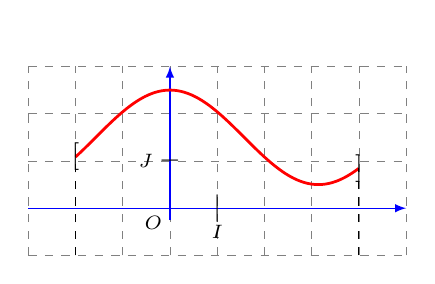
\begin{tikzpicture}[scale=0.6,>=latex]
    \draw[dashed,very thin,color = gray] (-3,-1) grid (5,3);
    \draw[->,blue] (-3,0)--(5,0);
    \draw[->,blue] (0,-0.25)--(0,3);
    \draw[color=red,line width=1pt] plot[domain=-2:4,samples=200] (\x,{cos(deg(\x))+1.5});
    \draw[dashed] (-2,-1)--(-2,{cos(deg(-2))+1.5});
    \draw[dashed] (4,-1)--(4,{cos(deg(4))+1.5});
    \draw (-2,{cos(deg(-2))+1.5}) node{\rouge{$[$}};
    \draw (4,{cos(deg(4))+1.5}) node{\rouge{$]$}};
    \draw (1,0) node {$|$};\draw (0,1) node {$-$};
    \draw (0,3.5) node {\textcolor{white}{a}};
    \begin{scriptsize}
        \draw (0,0) node[below left]{$O$};
        \draw (1,-0.2) node[below]{$I$};
        \draw (-0.2,1) node[left]{$J$};
    \end{scriptsize}
\end{tikzpicture}&
%-- colonne 2
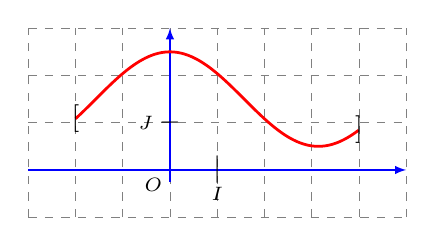
\begin{tikzpicture}[scale=0.6,>=latex]
    \draw[dashed,very thin,color = gray] (-3,-1) grid (5,3);
    \draw[->,blue] (-3,0)--(5,0);
    \draw[->,blue] (0,-0.25)--(0,3);
    \draw[color=red,line width=1pt] plot[domain=-2:4,samples=200] (\x,{cos(deg(\x))+1.5});
    \draw (-2,{cos(deg(-2))+1.5}) node{\rouge{$[$}};
    \draw (4,{cos(deg(4))+1.5}) node{\rouge{$]$}};
    \draw (1,0) node {$|$};\draw (0,1) node {$-$};
    \begin{scriptsize}
        \draw (0,0) node[below left]{$O$};
        \draw (1,-0.2) node[below]{$I$};
        \draw (-0.2,1) node[left]{$J$};
    \end{scriptsize}
\end{tikzpicture}&
%-- colonne 3
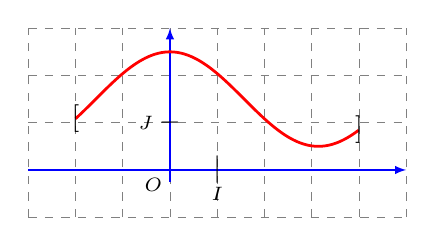
\begin{tikzpicture}[scale=0.6,>=latex]
    \draw[dashed,very thin,color = gray] (-3,-1) grid (5,3);
    \draw[->,blue] (-3,0)--(5,0);
    \draw[->,blue] (0,-0.25)--(0,3);
    \draw[color=red,line width=1pt] plot[domain=-2:4,samples=200] (\x,{cos(deg(\x))+1.5});
    \draw (-2,{cos(deg(-2))+1.5}) node{\rouge{$[$}};
    \draw (4,{cos(deg(4))+1.5}) node{\rouge{$]$}};
    \draw (1,0) node {$|$};\draw (0,1) node {$-$};
    \begin{scriptsize}
        \draw (0,0) node[below left]{$O$};
        \draw (1,-0.2) node[below]{$I$};
        \draw (-0.2,1) node[left]{$J$};
    \end{scriptsize}
\end{tikzpicture} \\
\hline
$\calig D_f =$ &
Image de $2,5$ : &
Antécédent(s) de $2$ :\par\bigskip
Antécédent(s) de $-1$ :\\
\hline
\end{tabularx}\bigskip

\subsection{À partir d'un tableau}
On considère la fonction $f$ définie de la façon suivante :

\begin{center}
\begin{tabular}{|*{6}{c|}}
\hline
$x$ & $-2$ & $-1$ & $0$ & $1$ & $2$ \\
\hline
$f(x)$ & $1$ & $3$ & $8$ & $10$ & $3$ \\
\hline
\end{tabular}
\end{center}\bigskip

\begin{description}
    \item[Ensemble de définition.] \strut\bigskip
    \item[Lecture d'image.] Image de $1$ :\bigskip
    \item[Lecture d'antécédents.] Antécédents de $3$ et de $2$ :
\end{description}\bigskip

\subsection{À partir d'une formule}
\begin{Rmq}
    Connaître une fonction $f$ à partir d'une formule explicite permet d'avoir de nombreux renseignements :
    \begin{itemize}
        \item on peut calculer l'image de n'importe quel nombre de l'ensemble de définition ;
        \item une formule permet de traduire le lien existant entre deux quantités.
        \item trouver un antécédent $a$ d'un nombre connu $b$ revient à résoudre l'équation $f(a) = b$.
    \end{itemize}
\end{Rmq}\medskip


Le poids idéal en fonction de la taille en $cm$ d'un homme et d'une femme adulte est calculé respectivement à l'aide des fonctions $h$ et $f$ ci-dessous :
\[h(t) = t - 100 - \dfrac{t - 150}{4} \qquad f(t) =  t - 100 - \dfrac{t - 150}{2,5}\]
\begin{enumerate}
    \item Quelles sont les deux quantités liées par chaque formule ? Quelle est celle qui dépend de l'autre ?
    \item Calculer le poids idéal d'un homme mesurant $1,75~m$.
    \item Calculer le poids idéal d'une femme mesurant $1,70~m$.
    \item Le nombre $59$ est-il l'image ou l'antécédent de $165$ par la fonction $f$ ?
    \item Calculer l'antécédent de $50$ par la fonction $f$ et interpréter le résultat.
\end{enumerate}



\end{document}
